% -*- mode: LaTeX; coding: utf-8; -*-

\chapter{Web-palveluiden haasteet}

Toimivan ja ennen kaikkea turvallisen web-pohjaisen palvelun tarjoaminen vaatii
nykyisin todella paljon aikaa ja huolellisuutta niin palvelun kehittäjältä kuin myös
palvelun tarjoajalta ja ylläpitäjältä. Ajat ovat muuttuneet huomattavasti siitä,
jolloin käyttäjät selailivat pääasiassa vain staattisia web-sivuja ja käyttivät tarjotuista
palveluista korkeintaan sähköpostia. Kehitys kulkee kovaa vauhtia eteenpäin, ja
tämän päivän suurimpia trendejä ovat ominaisuudet kuten interaktiivisuus,
sosiaalisuus ja yksilöllisyys, joiden avustuksella verkon käytöstä pyritään tekemään
käyttäjille entistä henkilökohtaisempi kokemus. Palvelut kuten MySpace,
Facebook ja YouTube ovat edelleen vahvistaneet näitä käyttäjätottumuksia, ja
markkinoille onkin syntynyt kova kilpailu siitä, kuka kehittää seuraavan
menestyspalvelun. Nykyisin puhutaankin internetin seuraavasta evoluutiosta Web 2.0:
n muodossa, joita myös edellä mainitut palvelut edustavat. Uudet teknologiat ja
kiire tuovat kuitenkin aina mukanaan joukon uusia heikkouksia, joita hyökkääjät
pyrkivät hyödyntämään. Suunnittelijan ja ylläpitäjien kannalta onkin tärkeää, että 
kehityksen tuomiin haasteisiin pyritään vastaamaan mahdollisimman nopeasti ja tehokkaasti.

\section{Mitä tarkoittaa Web 2.0?}

Web 2.0 on termi, jota käytetään hyvin monessa eri tarkoituksessa ja
asiayhteydessä. Se yhdistetään usein uusiin web-teknologioihin ja internet-
aikakauden tuotteiden/palveluiden kehityskaarien kuvaamiseen \cite{WEB2}. Yhteistä näille
on se, että ne pyrkivät esittämään sitä muutosta ja kasvua, jota internet pitää tällä
hetkellä sisällään. Tämä muutos on lähtöisin siitä, että kuluttajatottumukset
ovat kehittyneet kohti interaktiivisia palvelumalleja, joissa käyttäjillä on
entistä suurempi mahdollisuus vaikuttaa siihen, mitä informaatiota esitetään ja kuinka se esitetään.
Sosiaalisuus ja sen luoma yhteisöllisyys ovat luoneet tarpeen palveluille,
joissa käyttäjät pystyvät tekemään useita asioita saman aikaisesti saumattomasti
yhdestä paikasta käsin. Toinen kantava voima  muutokselle on ollut markkinoiden
tuoma paine, johon yritykset ovat pyrkineet mukautumaan niin kuluttajapuolella kuin myös
yrityspuolella. Tätä varten yritykset ovat kehittäneeet entistä suurempia ja 
monimutkaisempia kokonaisuuksia uusilla teknologioilla, joiden käyttöä ei aina riittävästi hallita. 
Tähän kun vielä lisätään kiire päästä markkinoilla ensimmäisten
joukossa, niin tietoturva jää usein taka-alalle \cite{WEB2b}.

Tietoturvan kannalta teknologiat, jotka luetaan kuuluvan osaksi Web 2.0
teknologiaperhettä, ovat jatkuvan huomion ja kehityksen kohteena. Nämä teknologiat
muodostavat sen voiman, joka mahdollistaa siirtymisen interaktiivisiin
sovelluksiin kuten Google Maps ja yritysten toiminnan siirtymisen verkkoon.
Teknologiat kuten Asynchronous JavaScript (AJAX), Cascading Style Sheet (CSS),
Flash, ActiveX ja XML voidaan kaikki laskea kuuluvan osaksi Web 2.0-perhettä.
Osa näistä teknologioista on ollut jo pidemmän aikaa käytössä, kun taas osaa on
vasta nyt alettu hyödyntämään siihen, mihin ne on alun perin suunniteltu \cite{WEB2}.
Kuvassa \ref{web} on nähtävillä näiden yleisimpien teknologioiden ja protokollien
väliset suhteet.

\begin{figure}[htp]
\centering
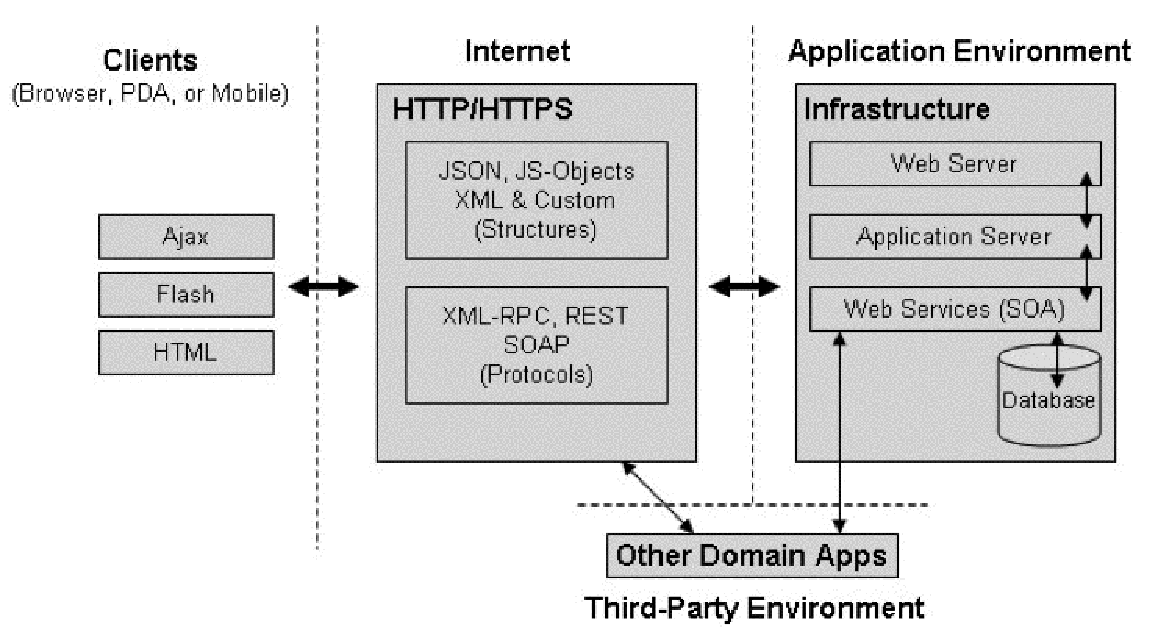
\includegraphics[width=12cm]{pics/web.pdf}
\caption{Web 2.0}
\label{web}
\end{figure}

Mitä Web 2.0 sitten tarkoittaa tietoturvan kannalta? Ensinnäkin se tuo mukanaan
samat vanhat haavoittuvuudet kuin mitä Web 1.0 sisälsi. Näiden lisäksi
hyökkäykset kuten Cross-site Scripting (XSS) ja Cross-site Request Forgery (CSRF) 
ovat aikaisempaa vaarallisempia, koska käytetyt teknologiat tarjoavat
rikkaamman ympäristön, jonka kautta murtautua järjestelmiin \cite{WEB2}. Web 2.0
sovellukset antavat myös loppukäyttäjälle ja takana oleville ohjelmille enemmän
valtaa, jonka johdosta loppukäyttäjä ei välttämättä edes huomaa joutuessaan
tietomurron kohteeksi. Otetaan esimerkiksi Ajax-teknologia, joka mahdollistaa
sivujen tietojen päivittämisen käyttäen asynkronisia kutsuja. Näiden ansiosta
käyttäjä pystyy tekemään kutsuja palvelimille ja päivittämään osan sivun
tiedoista niin, ettei koko sivua tarvitse päivittää. Tästä suurin osa tapahtuu
käyttäjältä piilossa, joten hän ei todennäköisesti huomaa, jos selain lataa
haitallisia skriptejä koneelle käyttäen jotain tunnettua haavoittuvuutta. Joidenkin
arvioiden mukaan jopa 70 prosenttia kaikista haitallisista koodeista ladataankin käyttäen
Ajaxia \cite{WEB2c}.

Palvelinpuolella muutokset eivät rajoitu vain Web 2.0 tuomiin
tietoturvariskeihin, sillä uudenlainen ajattelu vaatii myös uudenlaisen
palveluarkkitehtuurin. Uusi arkkitehtuuriratkaisu tuo aina mukanaan suuren
joukon muutoksia, jotka tulee ottaa huomioon tietoturvaa suunniteltaessa.
Palvelukeskeinen arkkitehtuuri (engl. Service Oriented Architecture, SOA) on
yksi näistä kehysmalleista, joka on kasvattanut suosiotaan Web 2.0:n
vanavedessä. SOA-arkkitehtuurilla onkin nykyisin tärkeä rooli palvelujen
välisen kommunikoinnin kehittämisessä. Siksi onkin tärkeää ymmärtää mistä
palasista SOA-arkkitehtuuriin perustuvat palvelut koostuvat, ja mitä tämä
tarkoittaa turvallisuuden kannalta.

\section{Palvelukeskeinen arkkitehtuuri}

Web-pohjaiset teknologiat ovat saamassa yhä suurempaa huomiota yrityspuolen
sovelluskehityksessä. Tätä muutosta on ollut ohjaamassa teknologioiden
kehittyminen siihen pisteeseen, jossa yritykset pystyvät tarjoamaan aikaisemmin
asiakas-serveri sovelluksia verkon välityksellä luotettavasti ja nopeasti. Tämä
ratkaisu on tuonut mukanaan rahallisia säästöjä yrityksille, jotka ovat ennen
joutuneet itse huolehtimaan mm. sovellusten ajan tasalla pitämisestä ja
palvelimien ylläpitämisestä \cite{WEB2}. Muutos on luonut myös tarpeen löytää yhä
tehokkaampia kehitysmalleja ja tapoja toteuttaa entistä monimutkaisempia ja
vaativimpia sovelluksia suuryritysten tarpeisiin. Yksi tapa hallita tätä
muutosta on perustaa tehdyt ohjelmistosuunnittelun ratkaisut palvelukeskeisen
arkkitehtuurin malliin.

Puhuttaessa web-palveluista palvelukeskeinen arkkitehtuuri lähtee siitä
ajatuksesta, että palveluiden toiminnot ja prosessit pyritään suunnittelemaan
toimimaan mahdollisimman itsenäisesti ja avoimesti siten, että niitä pystytään
kutsumaan joustavasti eri sovellusten välillä käyttäen standardoitua rajapintaa.
Tähän ratkaisuun ovat ajaneet pyrkimys laskea IT-kustannuksia ja jo käytössä olevien 
ratkaisujen uudelleenkäytön maksimointi. Aikaisemmin tämän toteuttaminen
on ollut vaikeaa sovellusten heterogeenisyyden takia, jonka johdosta eri
alustojen ja toimittajien väliset yhteistoiminnot ovat olleet usein mahdottomia
toteuttaa. Yhä useamman sovelluksen ja palvelun siirtyessä verkkoon tästä
halutaan nyt päästä eroon, ja tähän ongelmaan palvelukeskeinen arkkitehtuuri
pyrkii tuomaan ratkaisun. Käytännössä tämä tarkoittaa sitä, että arkkitehtuurin
tulee tarjota sovelluksille mahdollisimman joustava sekä sijainnista ja
protokollasta riippumattoman alusta \cite{SOA}. Tämän avulla loppukäyttäjälle
voidaan tarjota palveluita monesta eri paikasta yhtä aikaa siten, ettei hän ole
edes tietoinen tästä. Kyseessä on sama ajattelumalli johon Web 2.0 sovellukset
pohjautuvat, ja siksi palvelukeskeinen arkkitehtuuri onkin saanut paljon
nostetta Web 2.0:n myötä.

Palvelukeskeisen arkkitehtuurin tuomat edut eivät rajoitu pelkästään
kustannussäästöihin. Sen tuomiin etuihin kuuluvat myös mm. uusien toimintojen
helpompi integrointi jo käytössä oleviin järjestelmiin sekä monimutkaisten
kokonaisuuksien sujuvampi hallinta. Organisaatioille on myös tärkeää, että tällä
tavalla suunniteltuihin palvelumalleihin on nopeampi tehdä haluttuja muutoksia, jolloin 
reagointi markkinamuutoksiin voidaan toteuttaa nopeassa aikataulussa \cite{WEB2c}. Tämä on
erityisen tärkeää, koska markkinoille on ilmestynyt monia uusia tekniikoita,
jotka mahdollistavat web-palveluiden integroinnin jo käytössä oleviin
palveluihin. Onkin arvioitu, että vuonna 2008 web-pohjaisiin palveluihin
käytettiin jo yli 11 miljardia dollaria, ja osa fokuksesta on jo siirtynyt
kohti keskikokoisia ja pieniä yrityksiä. Web-pohjaisten palveluiden merkityksen
uskotaankin entisestään kasvavan ja yritykset, jotka reagoivat hitaasti tähän
muutokseen, huomaavat tulevaisuudessa olevansa epäsuotuisassa asemassa \cite{WEB2b}.

Palvelinpuolelle tapahtuva muutos tarkoittaa sopeutumista uudenlaiseen
ajattelumalliin, jossa palvelut on hajautettu ympäri verkkoa, ja joista osa ei
välttämättä ole saman ylläpitäjän hallinnassa. Kuvan \ref{soa} mukainen ratkaisu
tulee olemaan tulevaisuudessa arkipäivää, ja se tuo mukanaan uusia rajapintoja,
joiden kautta hyökkääjä voi pyrkiä murtautumaan järjestelmään tai jopa
yrityksen sisäiseen verkkoon. Koska palveluiden välinen kommunikointi perustuu
tässä mallissa luottamussuhteen luomiseen, tulee erityistä kiinnittää huomiota
siihen kuinka salaukset ja tunnistautuminen hoidetaan web-palveluita tarjoavien
osapuolien sekä käyttäjien kesken \cite{WEB2b}.

\begin{figure}[htp]
\centering
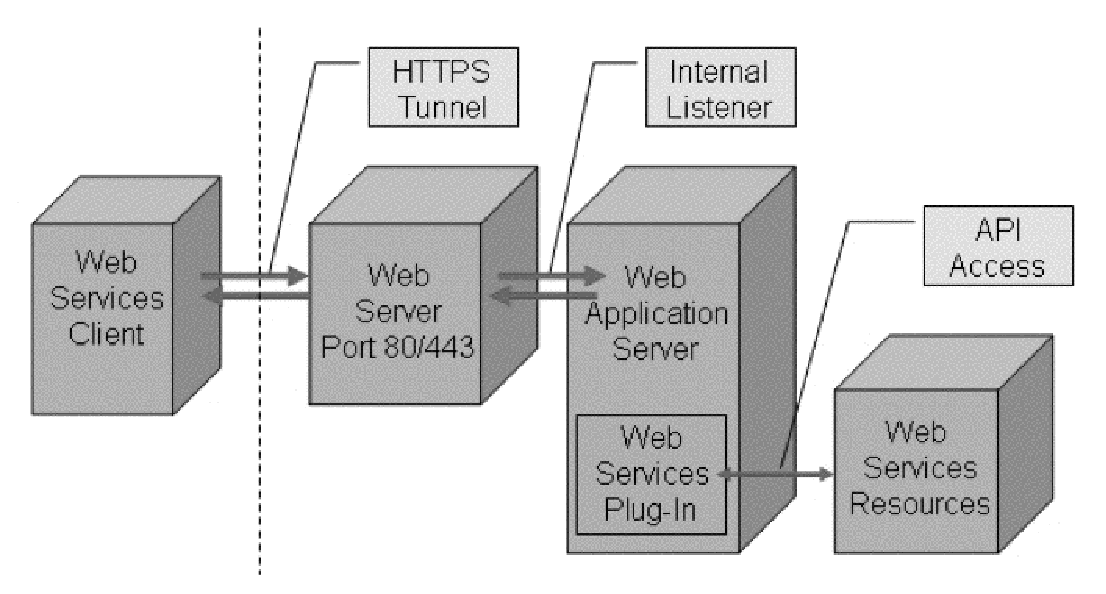
\includegraphics[width=12cm]{pics/soa.pdf}
\caption{SoA-arkkitehtuuri}
\label{soa}
\end{figure}

\section{Web-palveluiden tietoturva}

Internetin kehittyessä myös web-palveluihin kohdistuvat hyökkäykset ovat saaneet
uusia ilmenemismuotoja. Aikaisemmin ``web hakkerointia'' käytettiin kuvaamaan
hyökkäyksiä, jotka kohdistuivat palveluita tarjoaviin alustoihin kuten Apache, 
Microsoft IIS ja LAMP. Nämä hyökkäykset perustuivat tunnettujen haavoittuvaisuuksien
hyödyntämiseen, ja oikeille työkaluilla varustautunut hyökkääjä pystyikin kaatamaan haavoittuvan
palvelun muutamassa minuutissa. Esimerkiksi tunnetuimpien internet-matojen Code Redin ja Nimdan toiminta
perustui Microsoft IIS:sä olevan haavoittuvuuden hyödyntämiseen \cite{Hacking}. 

Tämänlaiset hyökkäykset ovat kuitenkin
menettäneet suurimman tehonsa, koska tehdyistä virheistä on opittu. Löydettyihin haavoittuvaisuuksiin
reagoidaan entistä nopeammin, yhä useampi alusta on konfiguroitu oikein ja saatavilla on työkaluja, joiden
avulla pystytään nopeasti ja helposti havaitsemaan yleisimmät tietoturvariskit \cite{Hacking}. Näistä seikoista johtuen
hyökkääjät ovatkin kiinnittäneet entistä enemmän huomiota itse alustalla pyöritettäviin palveluihin pyrkien 
murtautumaan järjestelmiin näiden kautta. Web 2.0:n myötä tämän tyyppiset hyökkäykset ovat saaneet entistä
enemmän huomiota, sillä se on tarjonnut hakkereille entistä monipuolisemman hyökkäyspinnan. Tietoturvan 
kannalta onkin tärkeää, että kumpaankin hyökkäystapaan kiinnitetään huomiota.

\subsection{Web-palvelimien turvaaminen}

Yllä mainitut seikat eivät tarkoita sitä, että web-palveluita pyörittävät alustat olisivat
turvassa hyökkäyksiltä. Onnistuneet hyökkäykset ovat edelleen yhtä tuhoisa, jos niihin ei varauduta ennalta.
Nämä erilaiset hyökkäykset pyrkivät yleensä hyödyntämään seuraavissa kategorioissa olevia heikkouksia

\begin{itemize}
\item Valmiit esimerkkitiedostot
\item Lähdekoodin paljastuminen
\item Kanonisointi
\item Palvelmiin asennetut lisäosat
\item Syötteen tarkistaminen \cite{Hacking}.
\end{itemize}
Tässä yhteydessä kanonisoinnilla tarkoitetaan sääntöjen mukaisen syötteen väärinkäyttöä. Hyökkäys pohjautuu siihen,
että useimpia palveluita ja resursseja voidaan kutsua monin eri tavoin. Esimerkiksi tiedostoa C:\textbackslash text.txt voidaan 
kutsua syntaksilla ..\textbackslash text.txt. Sovellukset, jotka tekevät tietoturvapäätökset käyttäen hyödyksi resurssinimeä,
voidaan helposti huijata suorittamaan odottamattomia toimintoja \cite{Hacking}.

Listatuilta asioilta suojautuminen on melko yksinkertaista, kunhan muistaa noudattaa muutamaa pääperiaatetta. Ensinnäkin tuotannossa 
olevilla palvelimilla ei tulisi koskaan olla asennettuna tai käytettynä tiedostoja, joiden turvallisuudesta ei ole
takeita. Näihin tiedostoihin kuuluvat mm. paketeissa mukana tulevat esimerkkitiedostot ja palvelimelle asennettavat 
lisäosat, joiden alkuperästä ei ole varmuutta. Toisekseen on tärkeä varmistaa, että käytettyihin sovelluksiin
on asennettu viimeisimmät päivitykset, sillä ne yleensä korjaavat tunnetut heikkoudet \cite{Hacking}. Jo pelkästään näillä 
toimilla pystytään suurimmaksi osaksi estämään sellaiset hyökkäykset, jotka kohdistuvat itse käytettyyn palvelinalustaan.
Palvelunesto- ja spoofing-hyökkäyksiltä nämä eivät kuitenkaan suojaa, ja tästä syystä resursseihin kohdistuville hyökkäyksille
tuleekin olla erilliset suojausmenetelmät.

\subsection{SQL injektio}

Virheelliseen syöttötietoon perustuvat hyökkäykset ovat jo pidemmän aikaa vaivanneet web-pohjaisia sovelluksia.
Web 2.0:n myötä hyökkäykset ovat entisestään yleistyneet, sillä monimutkaisten sovellusten takana käytetään entistä
enemmän erilaisia tietokantapohjaisia ratkaisuja kuten MySQL. Nämä hyökkäykset hyödyntävät sitä seikkaa, että suurin osa
sovelluksista ei tee selkeää eroa käyttäjän antaman syötteen ja ohjelmalle annettavien ohjeiden välillä. Tämä mahdollistaa
sen, että hyökkääjä pystyy piilottamaan annettuun hakuun ohjelmatason käskyjä, jotka muokkaavat sovelluksen toimintaa
hyökkääjän haluamaan suuntaan \cite{WEB2}. Normaaleilla toimenpiteillä tällaisen hyökkäysten tunnistaminen on hankalaa, sillä
yritysten tietoturvasta vastaavat palomuurit toimivat OSI-mallin kolmannella, neljännellä ja viidennellä kerroksella, eivätkä ne tunnista
ylimmän tason eli ohjelmistotason kautta tulevia hyökkäyksiä. Tämän lisäksi useimmat palomuurit eivät ymmärrä protokollien
kuten HTTP:n tarkkaa sisältöä \cite{SQLSS}.    

Onnistunut injektiohyökkäys koostuu kolmesta erillisestä vaiheesta. Ensimmäisessaä vaiheessa hyökkääjän tulee tunnistaa 
web-sovelluksessa käytetyt teknologiat. Tämä onnistuu mm. tulkitsemalla sivujen antamia virheilmoituksia, tutkimalla 
sivun lähdekoodia ja käyttäen tätä varten tehtyjä työkaluja kuten Nessus ja Nmap. Tämä vaihe on hyökkääjälle melko triviaali
tehtävä, mutta hyökkäyksen kannalta tiedot ovat elintärkeitä, sillä injektiohyökkäyksen onnistuminen on täysin riippuvainen 
käytetystä ohjelmointikielestä. Kun tarvittavat tiedot on saatu kerättyä, voidaan varsinaista hyökkäystä alkaa suunnittelemaan.
Tämä tapahtuu tunnistamalla ne syötteet, jotka käyttäjä pystyy sovellukselle antamaan. Tämä käsittää käytännössä kaiken sen 
datan, joka kulkee HTTP GET ja HTTP POST pyynnöissä. Viimeisessä vaiheessa hyökkääjän tehtäväksi sitten jää niiden syötteiden 
tunnistaminen, joita käyttämällä sovelluksen toimintaa saadaaan muokattua. Tähänkin tehtävään löytyy useita valmiita työkaluja, ja
monessa tapauksessa samat toimintaperiaatteet toimivat eri sovellusten välillä \cite{WEB2}.

Structured Query Language (lyh. SQL), joka on alan de facto standardi tietokantojen käsittelyyn, on käytössä lähes jokaisessa
web-sovelluksessa, joka käyttää jonkinlaista tietokantaratkaisua. Sen syntaksi on sekoitus ohjelmakäskyjä ja käyttäjän antamia
syötteitä, ja huonosti määritettynä käyttäjän antama syöte voidaan tulkita virheellisesti ohjelmatason käskyksi. Tämän syötteen
hyökkääjä joutuu usein etsimään sokeasti, mutta syötteet kuten

\begin{itemize}
\item ' OR 1=1 "{-}{-}
\item ') OR 1=1 "{-}{-}
\end {itemize}
toimivat hyvin usein \cite{WEB2}. Virheellisestä hausta aiheutuvat virheilmoitukset antavat myös erittäin paljon
hyödyllistä tietoa hyökkääjälle \cite{SQLSS}. Koska suurin osa SQL-tietokannoista mahdollistaa useamman perättäisen syötteen 
antamisen, kunhan syntaksi pysyy oikeana, voidaan näiden avulla katkaista ohjelman normaali toiminta. Otetaan esimerkiksi SQL-haku
\begin{tt}
\begin{center}
String query= ``SELECT id FROM user\_table WHERE `` + \\
``username = ' `` + username + ``' AND `` + \\
``password = PASSWORD(' `` + password + ``')''; \\
\end{center}
\end{tt}
Antamalla käyttäjänimeksi arvon

\begin{tt}
\begin{center}
' OR 1=1; DROP TABLE user\_table;"{-}{-}
\end{center}
\end{tt}
muuttuu tietokannalle ohjautuva kysely muotoon

\begin{tt}
\begin{center}
String query= ``SELECT id FROM user\_table WHERE username=' ' OR 1=1; DROP TABLE
user\_table; "{-}{-} ' AND password = PASSWORD ('x');
\end{center}
\end{tt}
SQL-kielessä kaksi perättäistä viivaa tarkoittaa, että kaikki siitä oikealla puolella oleva on kommenttia. 
Näin ollen lopullinen SQL-haku on 

\begin{tt}
\begin{center}
String query= ``SELECT id FROM user\_table WHERE \\username=' ' OR 1=1; DROP TABLE
user\_table;
\end{center}
\end{tt}
Näin muodostettu haku on syntaktisesti täysin oikea, ja se tyhjentää tietokannassa olevan user\_table tiedoston, joka pitää
sisällään järjestelmään tallennetut käyttäjät \cite{WEB2}. 

Vastaavanlaisia tekniikoita käyttäen hyökkääjä pystyy tekemään kaiken sen, joka pystytään esittämään SQL-kyselynä, ja johon ajettavalla
sovelluksella on riittävät oikeudet. Mielivaltaisten käskyjen antaminen, DLL tiedostojen luominen ja ajaminen ja tietokannan
sisällön lähettäminen jollekin toiselle internetissä olevalle palvelimelle ovat vain muutamia esimerkkejä toiminnoista, joita
onnistunut hyökkäys voi aiheuttaa \cite{SQLSS}.

Injektiohyökkäykset eivät rajoitu pelkästään SQL-kieleen, sillä useat eri tekniikat kuten XPath ja LDAP sisältävät vastaavanlaisia 
heikkouksia \cite{WEB2}. SQL-kieleen pohjautuvat hyökkäykset ovat kuitenkin kaikista yleisimpiä johtuen sen levinneisyydestä. SQL-kieleen
pohjautuvat ratkaisut sisältävät usein myös osan seuraavista ominaisuuksista, jotka mahdollistavat hyökkäysten tekemisen:

\begin{itemize}
\item Kommentoinnin mahdollistavat merkki: "{-}{-}.
\item Mahdollisuus suorittaa useita hakuja yhdellä kertaa käyttäen puolipistettä.
\item SQL-palvelimen antamat tarkat virheilmoitukset
\item Syötteen tyypin ehdoton kääntäminen -- kokonaisluvut käännetään mahdollisuuksien mukaan merkkijonoksi, jolloin hyökkääjän
             on helpompi arvata oikea syöte \cite{SQLSS}.
\end{itemize}

Esille tulleiden asioiden valossa on selvää, että SQL-kieleen pohjautuvat haavoittuvaisuudet ovat todellinen uhka yritysten tietoturvalle.
Tästä johtuen on tärkeää, että sovellusten turvallisuus pyritään takaamaan kaikin mahdollisin tavoin. Täysin turvallisen sovelluksen 
suunnitteleminen on kuitenkin lähes mahdoton tehtävä, mutta noudattamalla muutamia perusperiaatteita voidaan riskiä vähentää huomattavasti.
Vastaavasti myös palvelinpuolella SQL-injektiohyökkäykset tulee ottaa huomioon suunniteltaessa verkon tietoturvaratkaisuja.

Koska injektiohyökkäykset pyrkivät hyödyntämään syötteiden virheellistä tulkintaa, voi hyväksyttävien syötteiden rajoittaminen tuntua
helpolta ratkaisulta ongelmaan. Osittain tämä ratkaiseekin asian, mutta ongelmaksi muodostuu se, kuinka valita mikä syöte on hyväksyttävä
ja mikä virheellinen. Tämän valitsemiseen on useita eri tapoja kuten esimerkiksi sallia ainoastaan syötteet, jotka tiedetään etukäteen hyväksi
ja huonon syötteen riisuminen tai pois tiputtaminen. Näistä tavoista ensimmäinen on kaikista rajoittavin, koska tällöin syötteen jokainen 
merkki tarkistetaan, ja jos se ei ole sallittujen merkkien joukossa niin koko haku hylätään. Huonojen syötteiden riisuminen on myös vaikea
toteuttaa, koska harvoin pystytään määrittelemään mikä haku on huono ja mikä hyvä. Yksi hyväksi todettu tapa onkin rajoittaa tiettyjen
merkkien käyttöä siten, että merkin ollessa haussa mukana tämä muutetaan toiseen muotoon. Tämäkään ratkaisu ei ole täysin ongelmaton, ja siksi
viisainta onkin vain hylätä koko syöte, jos se ei vastaa odotettua syötettä \cite{SQLSS}.

Palvelinpuolella tulee myös ottaa huomioon muutamia asioita, joita seuraamalla voidaan huomattavasti parantaa yrityksen tietoturvaa.
Palvelinpuolen ratkaisuilla voidaan myös pienentää huonosti suunnitellun sovelluksen riskiä joutua injektiohyökkäyksen kohteeksi. 
Seuraava lista ei ole millään tavalla täydellinen ratkaisu ongelmaan, mutta se antaa osviittaa siitä, millä tavoin riskiä voidaan vähentää:

\begin{itemize}
\item SQL-palvelimen ajaminen pienillä käyttöoikeuksilla.
\item Sallia tallennettujen proseduurien ajaminen ainoastaan järjestelmän ylläpitäjille
\item Linkitettyjen palvelimien yksinkertaisten tunnistusten poistaminen
\item Määrittää palomuuri siten, että ainoastaan luotetut käyttäjät saavat ottaa yhteyden SQL-palvelimeen. Usein ainoat, joiden yhteydet 
      tulee sallia, ovat ylläpitäjät ja web-palvelut, joita tietokanta palvelee \cite{SQLSS}.
\end{itemize}

\subsection{Cross-site Scripting}
Nykyisin yhä useampi yritys on tietoinen verkon tarjoamista mahdollisuuksista ja sen mukana tulevista vaaroista. Yritykset ovat tämän johdosta
alkaneet panostamaan entistä enemmän tietoturvaan, ja harva toimiikin enää ilman kunnollista suojausta. Palomuurit ja hyökkäysten tunnistamiseen
ja estämiseen erikoistuneet sovellukset ovat myös kehittyneet viime vuosina niin paljon, että enää harva perinteinen hyökkäys toimii ilman
suuria muutoksia sen toteutustapaan. Tästä johtuen hakkerit ovat alkaneet omaksumaan yhä salamyhkäisempiä hyökkäystapoja, jotka pyrkivät kokonaan
ohittamaan perinteiset palomuurit. Web-pohjaiset sovellukset tarjoavat tähän erinomaisen alustan, ja Web 2.0:n myötä mahdollisuudet vain kasvavat
entisestään.

Cross-site scripting eli XSS-hyökkäykset eivät ole millään tapaa uusi hyökkäystyyppi, ja joidenkin arvioiden mukaan kahdeksan kymmenestä sivustosta on 
sille jollakin asteella alttiina. XSS-hyökkäykset ovat kuitenkin viime vuosina keränneet suurempaa huomiota hakkereiden keskuudessa, sillä Web 2.0 sovellusten
myötä yhä useampi näistä käyttää erilaisia tiedonlähteitä sisällön keräämiseen. RSS-feedit, widgetit, moduulit ja erilaiset JavaScript-pohjaiset komponentit 
tarjoavat kaikki hyökkääjälle monta mahdollisuutta, johon iskeä. Tähän kun vielä lisätään se, että sovelluksista monet päivittävät tietoja käyttäjän tietämättä, 
niin tilanteesta muodostuu entistä vaarallisempi \cite{WEB2b}. Tästä johtuen XSS-hyökkäykset muodostavat nyt ja tulevaisuudessa erittäin suuren riskin
tietoturvalle.

Painotuksen siirtyminen web-pohjaisiin hyökkäyksiin on ollut selkeästi havaittavissa jo pidemmän aikaa. Vuonna 2007 johtava tietoturva-alan 
yritys Symantec julkisti raportin, jonka  mukaan vuoden 2007 viimeisen kuuden kuukauden aikana raportoiduista haavoittuvaisuuksista 11,253
oli sivustokohtaisia cross-site scripting tietoturva-aukkoja. Tätä lukua kun vertaa muihin löydettyihin riskeihin, joita oli 2,134, niin 
yli 80 prosenttia löydetyistä tietoturva-aukoista oli web-pohjaisia \cite{SYM}. Vuonna 2009 julkistetussa raportissa tilanne on edelleen sama, 
sillä 63 prosenttia haavoittuvaisuuksista kohdistui Web-sovelluksiin \cite{SYM2}.

Kuten aikaisemmin on jo tullut esille, niin injektiohyökkäykset eivät rajoitu pelkästään tietokantasovelluksiin. Myös XSS-hyökkäykset ovat eräänlaisia 
injektiohyökkäyksiä sillä erotuksella, että hyökkääjä ei suoraan toteuta injektiota vaan uhri tekee sen itse. Tähän hyökkääjällä on useita eri 
keinoja, ja harvoin käyttäjä edes huomaa joutuneensa hyökkäyksen kohteeksi. Hyökkäyksen onnistuessa web-sivujen käyttämä ``saman alkuperän'' periaate
voidaan kiertää, jolloin hyökkääjän on mahdollista ajaa kohteen selaimessa haluamaansa koodia ja skriptejä. Tämä ``saman alkuperän'' periaate on 
web-selainten yksi tärkeimmistä suojausmenetelmistä, ja se estää mm. skriptien lataamisen yhdestä lähteestä hakemalla tai asettamalla määrityksiä 
toisesta lähteestä \cite{WEB2}. Hyökkäys voidaan esimerkiksi toteuttaa siten, että haavoittuvalle web-sivustolle asennetaan vihamielinen skripti.
Tämä skripti on usein kirjoitettu JavaScriptillä, ja käyttäjän vieraillessa sivustolla se ajetaan käyttäjän web-selaimessa. Koska selain luottaa siihen, 
että sivuston sisältö on luotettavasta lähteestä, pystyy hyökkääjä lukemaan ja muokkaamaan arkaluontoista sisältöä. Evästeet, jotka ovat web-sovellusten 
toiminnan kannalta erittäin tärkeitä, ovat ensimmäisiä kohteita, joihin yritetään yleensä päästä käsiksi,  sillä ne pitävät yllä yhteyksien tiloja eri 
sivustoille ja oikean käyttäjän tunnistamiseen tarvittavia tietoja \cite{WEB2b}. Näitä kaappaamalla hyökkääjä pystyy esiintymään verkossa toisena käyttäjänä, 
ja väärinkäyttämään palveluita kuten verkkopankkia tai webmailia. Hyökkäys voidaan myös toteuttaa huijaamalla käyttäjä klikkaamaan vihamielistä linkkiä, 
joka aktivoi HTML-pohjaisen skriptin \cite{WEB2}.

Hyökkääjän mahdollisuudet eivät rajoitu pelkästään evästeiden varastamiseen. Onnistuneen XSS-hyökkäyksen jälkeen hakkeri voi esimerkiksi ohjata
käyttäjän osoitteeseen, joka jäljittelee haluttua sivustoa. Käyttäjän sitten yrittäessä kirjautua palveluun, saa hyökkääjä selville käyttäjän tunnuksen ja
salasanan. XSS-hyökkäykset tarjoavatkin erinomaisen mahdollisuuden toteuttaa phishing eli tiedon kalasteluhyökkäyksiä. XSS-madot ovat
myös viime aikoina yleistyneet, sillä yhä useampi palvelu on niille haavoittuvainen. Esimerkiksi webmail-sovelluksia varten kirjoitetut madot 
käyttävät hyödyksi sitä seikkaa, että hyökkääjä pääsee käsiksi uhrin kontaktilistaan. Tällainen mato pyrkii leviämään lähettämällä 
kontaktilistalla oleviin osoitteisiin sähköpostia, ja koska viesti tulee luotettavasta osoitteesta, ei käyttäjät osaa usein varoa viestissä
olevaa linkkiä. Hyökkääjä vielä usein muokkaa linkistä sen näköisen, että vastaanottaja ei osaa epäillä linkin aitoutta \cite{WEB2}. 
XSS-madot leviävätkin usein todella nopeasti, ja ne kuljettavat usein myös muita hyökkäyksiä mukanaan. Tästä hyvänä esimerkkinä
Sammy-madoksi nimetty XSS-hyökkäys, joka vuonna 2005 iski MySpace-sivustolle, joka on yksi tunnetuimmista sosiaaliseen verkoistutumiseen
erikoistuneista sivustoista. Käyttäen sivustossa olevaa heikkoutta hyväkseen mato saastutti käyttäjien sivuja, ja jonkun vieraillessa 
saastuneella sivulla, saastui myös hänen oma MySpace sivunsa. 24 tunnissa mato oli saastuttanut yli miljoona sivua, ja tilanteen korjaamiseksi
MySpace joutui sulkemaan sivustonsa. Hyökkäyksen vahingot eivät rajoittuneet tähän vaan seuraavina viikkoina useista tunnetuista sivustoista
kuten Google ja Yahoo löytyi vastaavanlaisia heikkouksia \cite{WEB2b}.

Tärkein asia XSS-hyökkäysten estämiseksi on olla hyvin tarkkana sen suhteen, kuinka käyttäjien tarjoama sisältö välitetään toisille käyttäjille.
Tärkeää on myös muokata käyttäjän antama syöte aina sellaiseen muotoon, että kun palvelin lähettää esimerkiksi virhesanomassa käyttäjän antaman syötteen
takaisin, niin ei tätä voida käyttää sellaisenaan hyökkäyksen toteuttamiseen. Tiettyjen merkkien poistamisella voitaisiin hyökkäyksi vähentää,
mutta usein merkkien kuten heittomerkin (') poistaminen ei tule kyseeseen. Suunnittelijoiden avuksi on myös olemassa suuri määrä sovelluksia, jotka
etsivät sivustoilla olevia heikkouksia \cite{WEB2}. Tämän suhteen tulee kuitenkin muistaa, että myös hakkereilla on käytettävissä samat sovellukset, joten 
löydetyt heikkoudet tulisi korjata mahdollisimman nopeasti. Symantecin raportin mukaan näin kuitenkin tapahtuu todella harvoin, sillä 6,961 
sivustosta vain 473 oli korjattu raportin kirjoittamisen aikana ja tähänkin oli mennyt keskimäärin 52 päivää \cite{SYM}. XSS-haavoittuvista sivuista
kirjaa pitävän sivuston mukaan tilanne ei ole nykyisin yhtään sen parempi, sillä suurin osa löydetyistä sivuista on edelleen korjaamatta \cite{XSS}.
Näyttääkin siltä, että yritykset ymmärtävät asian vakavuuden vasta sitten, kun sivusto on joutunut hyökkäyksen kohteeksi.

\subsection{Cross-site Request Forgery}

Web 2.0 sovellusten yksi keskeisimmistä asiakaspuolen ratkaisuista on Document Object Modeliksi (lyh. DOM) nimetty ohjelmointirajapinta, joka on vastuussa siitä, 
kuinka web-sivun sisältöä käsitellään ja kuinka eri objektit kommunikoivat keskenään. Rajapinta vastaa siitä, että ainoastaan saman domainin 
sisäinen kommunikointi ja sisällön muokkaaminen on sallittua. Tämä ratkaisu poistaa sen mahdollisuuden, että web-sivun DOM:ia voitaisiin muokata toisen
domainin kautta. Tämä vastaa ``saman alkuperän'' periaatetta, jolla pyritään estämään web-sivuihin ja käyttäjiin kohdistuvia vihamielisiä toimia.
Webin muuttuessa entistä interaktiivisemmaksi, ovat sivut kuitenkin alkaneet sallia yhä enemmän domainien välistä kommunikointia. Tällaisia 
toimia ovat esimerkiksi hyperlinkkien käyttäminen sisällön näyttämisessä, kuvien ja objektien lataaminen sekä toisessa domainissa olevien 
JavaScriptien ajaminen. Nämä ja monet muut toimet ovat mahdollistaneet entistä monipuolisempien web-palveluiden suunnittelun, mutta huonosti toteutettuna 
ne jättävät palvelut hyvin haavoittuviksi. Tämä johtuu siitä, että käyttäjän tarkoituksella tekemiä toimia ei pystytä erottamaan niistä toimista, jotka tehdään 
automaattisesti käyttäjän vieraillessa sivustolla \cite{WEB2}.

XSS-hyökkäysten tapaan myös Cross-site Request Forgery (lyh. CSRF) hyökkäykset ovat jo pidemmän aikaan olleet olemassa, mutta vasta Web 2.0:n myötä ne
ovat alkaneet yleistymään. Ero näiden kahden hyökkäyksen välillä on siinä, että missä XSS skripti suoritetaan käyttäjän selaimessa, niin CSRF hyökkäyksessä käytetyt
käskyt ja skriptit kohdistetaan luotettuihin web-palveluihin. CSRF toteutetaan siten, että hyökkääjä asettaa jollekin sivulle vihamielisiä tageja, joiden
avulla voidaan luoda mielivaltaisia HTTP pyyntöjä. Nämä pyynnöt sitten kohdistetaan johonkin toiseen domainiin, ja ne ajetaan käyttäjän vieraillessa kyseisellä 
sivulla. Jos käyttäjän selaimella on sitten esimerkiksi tähän domainiin liittyvä eväste voimassa, voidaan HTTP pyynnöillä pyytää mm.  salasanan vaihtoa 
tai sähköpostin lähettämistä käyttäjän nimissä \cite{WEB2b}. Hyökkääjä pystyy tällä tavoin myös ottamaan yhteyttä sellaisiin koneisiin ja palveluihin, joihin 
hänellä ei muuten olisi oikeuksia johtuen esimerkiksi palomuurista tai IP-osoitteiden suodatuksesta \cite{CSRF}.

CSRF hyökkäysten teho perustuu siihen, että monet sivustot ja palvelut käyttävät evästeitä melko huolimattomasti. Koska näiden avulla sivustot autentikoivat tulevat 
HTTP pyynnöt niin riittää, että hyökkääjä pääsee niihin käsiksi tavalla tai toisella. Useat sivustot myös sallivat käyttäjien pysyvän kirjautuneena sisällä
jopa useita viikkoja, jolloin sama eväste on pitkään käytössä. Monien sovellusten ja pyyntöjen rakenne on myös hyvin ennalta arvattavissa, jolloin hyökkääjän
on helpompi arvata käskyjen ja parametrien oikea muoto \cite{WEB2}.

CSRF hyökkäykset eivät rajoitu pelkästään perinteisiin web-tekniikoihin, sillä suurin osa Web 2.0:n mukana tuomista teknologioista on sille jollakin 
tavalla alttiina. Erityisesti AJAX ja JavaScript ovat tuoneet mukanaan suuren joukon uusia haasteita, jotka suunnittelijoiden tulee ottaa huomioon uusien
sovelluksien suunnittelussa. \cite{WEB2b}. Täydellinen suojautuminen CSRF hyökkäyksiltä vaatiikin sellaista syvällistä osaamista käytetyistä tekniikoista ja 
tietämystä eri komponenttien välisistä toimininnoista, jota harvalta löytyy. Siksi iso osa sivustoista ja palveluista onkin haavoittuvaisia eri asteisille
CSRF hyökkäyksille. Tästä hyvänä esimerkkinä tunnettu sähköpostisivusto Gmail, josta löytyi vuonna 2007 CSRF hyökkäyksen mahdollistava heikkous. Tämän avulla
hyökkääjän oli mahdollista luoda Gmailiin sellainen suodatus, joka ohjasi tulevat postit toiseen osoitteeseen \cite{CSRF}. 

CSRF hyökkäyksiltä suojautumiseen on käytössä kolme hyvin yleistä tekniikkaa. Näistä käytetyin on sisällyttää jokaiseen serveripuolen dataa muokkaavaan
GET/POST pyyntöön mukaan salattu tokeni, jonka avulla jokainen pyyntö voidaan yksilöidä ja tunnistaa kuuluvan oikeaan istuntoon. Tämä salattu tokeni tekee
käyttäjän syötteestä arvaamattoman muotoisen, jonka johdosta CSRF-hyökkäyksen toteuttaminen on hyvin vaikeaa \cite{WEB2}. Yksinkertaisin suojausmenetelmä on 
taas tunnistaa HTTP pyynnön Referer otsake, ja hyväksyä vain sellaiset pyynnöt, jotka tulevat luotettavista lähteistä. Kolmas menetelmä on tehdä kustomoituja
otsakkeita käyttäen XMLHttpRequestia, jonka käyttö on lisääntynyt AJAXin yleistyessä. Kustomoitujen otsakkeiden oikeellisuus sitten varmistetaan, ennen kuin
pyynnöt käsitellään palvelinpuolella \cite{CSRF}.

Nämä kolme esitettyä tapaa ovat yleisimmin käytössä, mutta nekin sisältävät joukon heikkouksia. Salatun tokenin ongelma on siinä, että kyseisestä tekniikasta ei 
ole olemassa yleisesti sovittua toteutustapaa. Tämä aiheuttaa sen, että useat ratkaisut ovat tavalla tai toisella puutteellisia. Referer otsakkeiden suodatuksen 
ongelma on siinä, kuinka käsitellä pyyntöjä, joista puuttuu Referer otsake. Otsakkeen piilottaminen ei ole vaikea tehtävä, joten palvelin saattaa joutua 
päättämään vajailla tiedoilla päästääkö pyyntö läpi vaiko suodattaa se pois. XMLHttpRequestin käyttöä taas rajoittaa sen tuomat lisävaatimukset toteutukselle,
joka rajoittaa tiettyjen palveluiden käyttöä \cite{CSRF}. 

Näiden ja monien muiden syiden takia tutkimustyö CSRF hyökkäysten parissa on kasvattanut suosiotaan. Esimerkiksi yhdessä tutkimuksessa ehdotettiin erillisen Origin
otsakkeen lisäämistä pyyntöön, joka korjaisi Referer kentän heikkoudet \cite{CSRF}. Toisessa tutkimuksessa taas pyrittiin kasvattamaan web-selaimen turvallisuutta
lisäämällä selaimeen mekanismi, joka pyrki arvioimaan vastasiko tehdyt pyynnöt käyttäjän toimia \cite{CSRFb}. Näistä kahdesta ratkaisusta on kuitenkin nähtävissä se,
että tutkimuskenttä CSRF hyökkäysten ympärillä on vielä hyvin alkuvaiheessa, ja vastuu riittävän suojauksen hoitamisesta jääkin vielä tällä hetkellä 
sovelluksen kehittäjälle ja ylläpitäjälle.

\section{Web-palveluiden turvaaminen}

Web-palveluiden tietoturvasta vastaaminen on tarkkuutta ja aikaa vaativaa työtä, joka edellyttää omien tietojen jatkuvaa päivittämistä sekä ja liikenteen ja palveluiden
seuraamista. Jo pelkästään yleisimpien tietoturvariskien tunnistaminen ja korjaaminen osoittautuu usein käsin tehtynä ylivoimaiseksi tehtäväksi verkkojen ja palveluiden
muuttuessa entistä monimutkaisemmiksi. Onneksi työn helpottamiseksi on saatavilla useita erilaisia työkaluja, joiden avulla sekä kehittäjät että ylläpitäjät voivat
etsiä sovelluksista ja verkoista tunnetuimpia tietoturva-aukkoja. Osa näistä pohjautuu vapaaseen lähdekoodiin, mutta tarjolla on myös kaupallisia sovelluksia, jotka ainakin 
paperilla lupaavat parempia ominaisuuksia. Näiden lisäksi myös palvelinpuolella on tarjolla erilaisia lisäosia, jotka lisäävät web-palveluiden tietoturvaa. 
Mikään sovellus ei tietenkään voi löytää kaikkia mahdollisia heikkouksia, joten pelkästään näiden varaan ei voi tietoturvaa rakentaa. Näiden avulla 
saadaan kuitenkin hyvä yleiskuva siitä, minkälaisille heikkouksille sovellus on mahdollisesti alttiina ja kuinka verkon turvallisuutta voitaisiin parantaa. Koska samat 
sovellukset on myös hyökkääjien käytössä, niin ainakin virheet, jotka löytyvät yleisimmin käytössä olevilla työkaluilla, tulisi korjata mahdollisimman nopeasti. 

Web Application Security Consortium (lyh. WASC) on vuonna 2004 perustettu avoin kansainvälinen ryhmittymä, joka koostuu tietoturva-alan asiantuntijoista sekä eri 
yritysmaailman tahoista, joiden tavoitteena on tuottaa vapaaseen käyttöön ``best-practice'' malleja ja standardeja turvallisesta internetistä. Se julkaisee
erilaisia artikkeleita, esitysmateriaaleja ja tietoturvalinjauksia, joita käytetään hyvin laajalti ohjenuorina yritysmaailmassa sekä tuotekehityksessä \cite{WASC}.
WASC:n tämän hetkisiin projekteihin kuuluvat mm. web-sovellusten turvallisuuden tutkimiseen käytettävien ohjelmistojen arviointikriteerien laatiminen sekä tilastointi
web-sovellusten turvallisuudesta. Viimeisimmän WASC:n tekemän raportin mukaan tutkituista sivustoista, joita oli yhteensä 12186 kappaletta ja joista löytyi 97554 
eri asteista tietoturvariskiä, 13 prosenttia pystyttiin murtamaan täysin automaattisesti, ja noin 49 prosenttia web-sovelluksista sisälsi helposti havaittavia vakavia 
tietoturvariskejä. Tämä luku kasvoi jopa 96 prosenttiin, kun sivuston tutki tietoturva-alan asiantuntija. Huomattavaa oli myös se, että sivustoista 99 prosenttia
ei noudattanut alan standardeja, ja ylläpidon aiheuttamat haavoittuvaisuudet olivat 20 prosenttia yleisempiä kuin sovellusten kehittäjien tekemät. Tutkimus myös 
osoitti sen, että XSS-hyökkäykset olivat SQL injektiohyökkäysten ohella kaikista yleisimpiä \cite{WASCb}. Tämän tiedon valossa onkin tärkeää, että sekä sovelluksen
kehittäjä että ylläpitäjä ovat ajantasalla sivuston/palvelun nykyisestä tilasta. 

\subsection{Nikto}

Nikto \cite{Nikto} on avoimeen lähdekoodiin perustuva ilmainen web-skanneri, joka etsii sivustoilta haavoittuvia CGI skriptejä ja tiedostoja. Sen tietokanta käsittää
yli 3500 tunnettua haavoittuvuutta sekä yli 900 eri web-alustoihin liittyvää heikkoutta. Nikto on koodattu käyttäen Perliä, ja se pyrkii skannaamaan palvelimen 
mahdollisimman lyhyessä ajassa. Tästä syystä sen aiheuttama liikenne on helppo havaita logeista. Tämän kiertämiseksi Niktoon on lisätty mahdollisuus käyttää Whiskerin
tarjoamaa libWhisker kirjastoa, joka pyrkii ohittamaan käytössä olevat suojausjärjestelmät. Nikto on erittäin tehokas ja käytetty työkalu perusturvallisuuden 
varmistamiseen, ja vuonna 2006 tehdyn tutkimuksen mukaan se valittiin parhaimmaksi web--haavoittuvaisuuksia skannaavaksi sovellukseksi \cite{INS}.
Nikton tietokantoja ei ole enää hetkeen päivitetty, joten nykyisellään se ei tunnista kaikista uusimpia hyökkäyksiä. Tästä huolimatta se on erittäin tehokas työkalu 
tietoturvan parantamiseen.

\subsection{Nessus}

Nessus \cite{Nessus} oli alunperin vapaaseen lähdekoodiin perustuva ilmainen tietoturvaskanneri, joka muuttui maksulliseksi vuonna 2008. 1200 dollarin vuosimaksua vastaan
saa kuitenkin yhden parhaimmista UNIX- ja Windows-alustoilla toimivista tietoturvaskannereista \cite{NST}. Se sisältää yli 20000 erillistä lisäosaa,
ja sen avulla on mahdollista suorittaa mm. reaaliaikaista liikenteen tarkkailua, konfigurointitiedostojen auditointia sekä eri verkko-osien skannausta. Maksullisuuden 
ansiosta Nessus pystytään pitämään ajantasalla uusimmista hyökkäyksistä, ja se soveltuukin erinomaisesti suurten ja monimutkaisten verkkojen turvaamiseen\cite{Nessus}. 

\subsection{Paros Proxy}

Paros Proxy \cite{Paros} on Javalla kirjoitettu web proxy, jonka avulla voidaan arvioida web-sovelluksen turvallisuutta. Se mahdollistaa kokonaisten sivustojen indeksoimisen,
jonka lisäksi sen avulla on mahdollista tallentaa ja muokata reaaliajassa käyttäjän ja palvelimen välistä HTTP ja HTTPS liikennettä mukaanlukien evästeitä. Sen mukana tulee
myös skanneri yleisimpien web-haavoittuvuuksien tunnistamiseen. Paros pohjautuu vapaaseen lähdekoodiin, ja se on hyvin käytetty työväline tietoturva-ammattilaisten
parissa, jotka etsivät sivustoilta haavoittuvuuksia.

\subsection{ModSecurity}

Koska nykyisistä hyökkäyksistä yhä useampi kohdistuu verkon laitteiden ja resurssien sijasta web-palveluihin ja -sovelluksiin \cite{WASCb} \cite{SYM}, eivät perinteiset
tietoturvaratkaisut pysty enää tarjoamaan riittävää tietoturvatasoa. Tästä syystä sovelluskehittäjät ja ylläpitäjät ovat joutuneet etsimään uusia ja entistä tehokkaampia 
tapoja hyökkäysten tunnistamiseen ja torjumiseen. Yksi mahdollinen ratkaisu on lisätä erillinen, web-sovelluksia varten suunniteltu palomuuri, käyttäjän ja palvelimen 
välille, jolloin palvelulle tulevat pyynnöt kulkevat tämän palomuurin kautta. Tällä tavoin saapuva liikenne voidaan tutkia ja suodattaa käyttäen haluttuja määrityksiä. 

ModSecurity \cite{Mod}on Apachelle suunniteltu, vapaaseen lähdekoodiin pohjautuva palomuuri, joka tarjoaa kattavan suojan web-palveluihin kohdistuvilta hyökkäyksiltä. 
Se mahdollistaa mm. HTTP liikenteen monitoroinnin ja reaaliaikaisen liikenteen analyysin vaatien korkeintaan hyvin pieniä muutoksia jo olemassaolevaan arkkitehtuuriin.
ModSecuritystä on saatavilla kaupallisia lisenssejä sekä eri asteisia tukipalveluita, mutta sovelluksen käyttämät perussäännöt ovat ilmaiseksi ladattavissa, vaikkakin näitä
ei ole hetkeen päivitetty. ModSecurityn käyttämä säännöstä mahdollistaa kuitenkin uusien sääntöjen kirjoittamisen omien tarpeiden mukaan, joten käytetyt säännöt voidaan räätälöidä 
omien tarpeiden mukaan \cite{Mod}. 

ModSecurityn parhaimpiin ominaisuuksiin kuuluu mahdollisuus ylläpitää täydellistä logia koko HTTP-tapahtuman ajalta, jolloin sekä pyynnöt että vastaukset pystytään analysoimaan.
Tämän ansiosta myös tulevien POST pyyntöjen sisältö ja rakenne voidaan tutkia. Nämä pyynnöt jäävät normaalisti logittamatta, ja tästä syystä iso osa hyökkäyksistä toteutetaankin 
nykyisin näitä käyttämällä. Se, mitä halutaan logittaa, voidaan myös tarkkaan määrittää. Salattu ja pakattu liikenne ei myöskään aiheuta ongelmia, sillä logitus tapahtuu sillä tasolla,
jossa pyynnöt ovat valmiiksi puretussa muodossa \cite{Mod}.

Liikenteen kirjaamisen ohella ModSecurity voidaan asettaa estämään tulevia hyökkäyksiä, jonka lisäksi sen avulla pystytään nopeasti paikkaamaan löydetyt haavoittuvaisuudet. 
Ensinnäkin kaikki tulevat paketit voidaan pisteyttää halutulla tavalla, ja tietyn pisterajan ylittäneet paketit voidaan esimerkiksi pudottaa pois. Toinen mahdollisuus on sallia vain 
tietynlaiset pyynnöt. ModSecurityn käyttämä säännöstökieli mahdollistaa myös palveluiden nopean suojaamisen uusilta hyökkäyksiltä ilman, että palvelun omaan koodiin tarvitsee koskea.
Tämä on erityisen hyödyllistä niissä tilanteissa, joissa päivitysten tuominen tuotantoon vie aikaa. 


